\section{讲解笔记：【第9次作业笔记】 位移计算(1)}
\begin{analysisbox}
本节按题目、答案和讲解笔记顺序整理。对扫描图中的结构几何关系，正文保留 OCR 可识别文字，并在图形页中保留清理后的题图，便于核对杆件、支座、荷载和尺寸。
\end{analysisbox}
\subsection*{第 1 页转写}
EA

【例4-49】图4-42（a）所示结构AB杆件EI,=oo，其余受弯杆件EI=常数，二力

杆抗拉刚度为EA，弹簧刚度k=3EI/256，试求C点的竖向位移。（北京交通大学2012）

AQ

120kN-m

AB：Jopdy

p-o

(*+

20kN

一创(二$\times$ 4x 40x 43)

4m

4m

2m

2m

4m

2m

4m

2m

4-1

图4-43所示结构中截面A转角（设顺时针为正）为（C）。（哈尔滨工业大学

2009)

A.2Fpa/EI

B. -Fpa?/EI

C.5Fpa /(4EI)

D.-5Fpa /(4EI)

图4-44所示悬臂梁，B点的竖向位移为

4-2

（合肥工业大学2010）

Fp=ql

2E1

EI

图4-43

图4-44

2EI

(2)

[1x(59 +]0x]单 +(1 4 *)
\begin{figure}[H]\centering
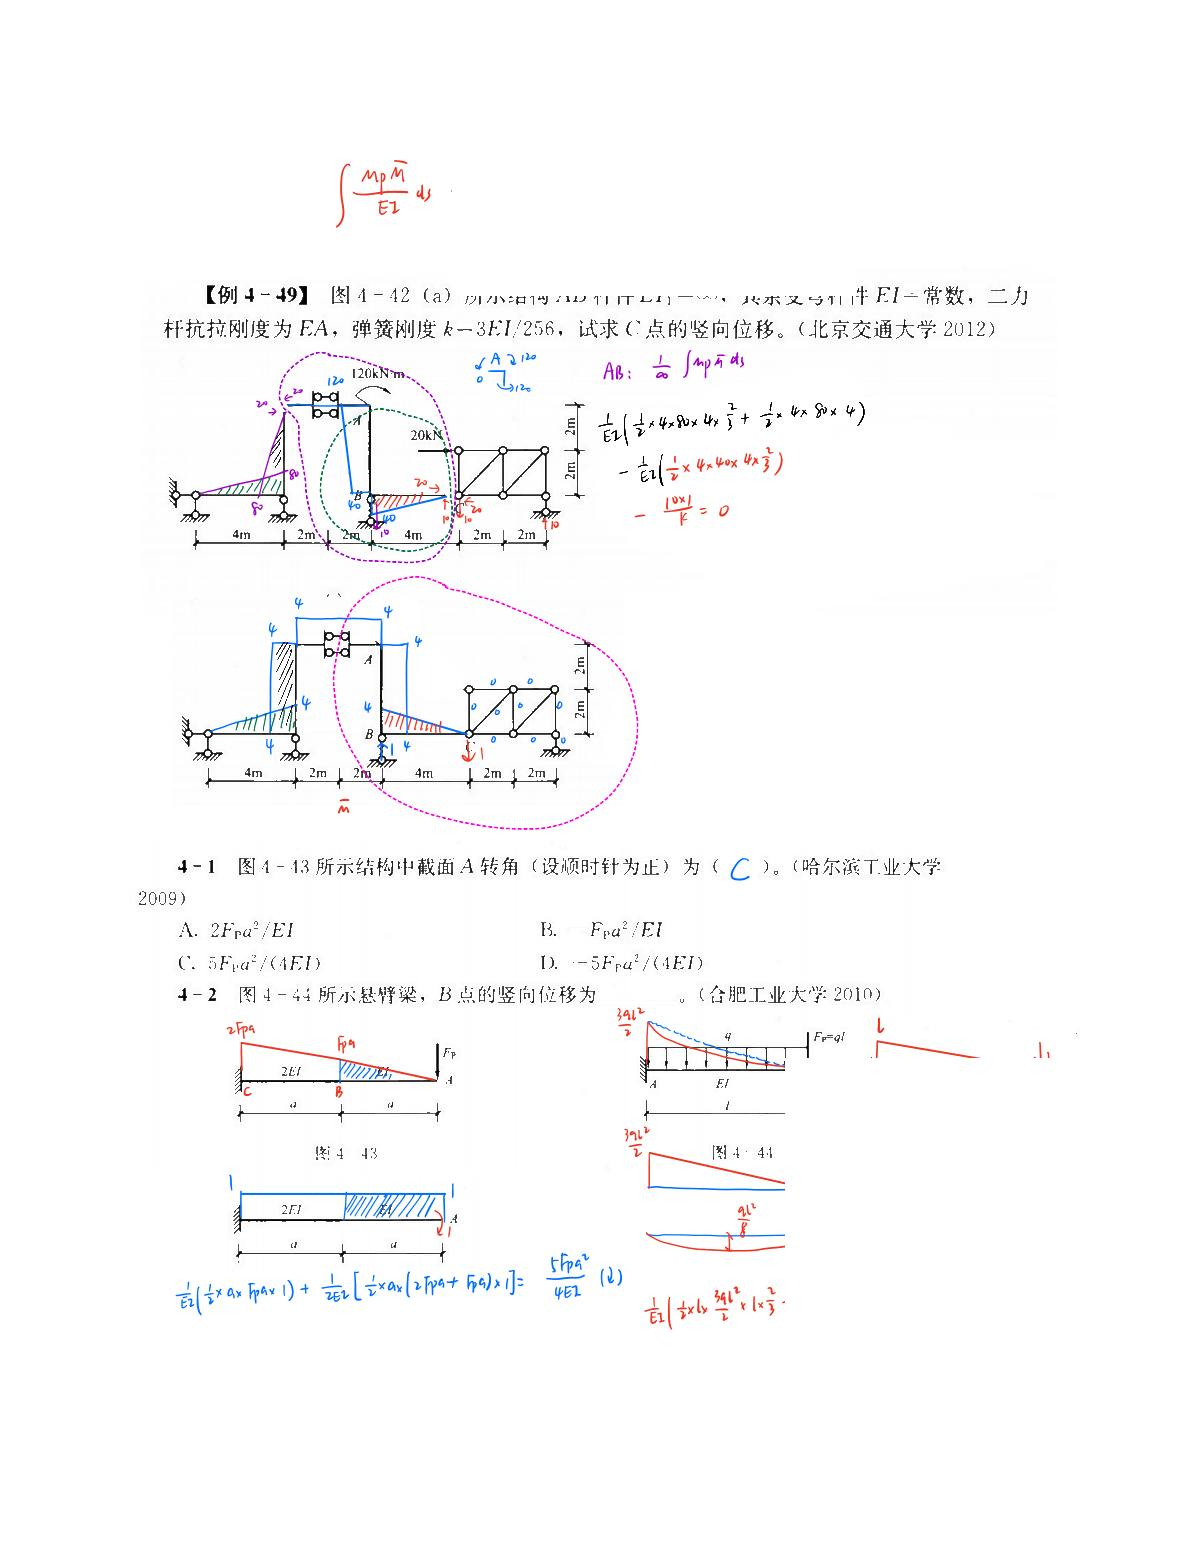
\includegraphics[width=0.92\textwidth]{figures/src29_p001.jpg}
\caption{【第9次作业笔记】 位移计算(1) 第 1 页清理图形页}
\end{figure}
\subsection*{第 2 页转写}
4-3图4-45所示桁架，C点的水平位移（D）。（西南交通大学2008）

A.向左

B.向右

C.等于零

D.不定，取决于A/A2的值

4-4图4-46所示刚架中，C、D两点的相对线位移等于

两点距离

 。（河北工业大学2010）

4-5图4-47所示架，各杆拉伸刚度为EA，DC杆的转角为

（天津大学

2010)

Fa. in82s]

ZMa=0.4a=p4+p39

EA

EA

EA2

(2)

FP

图4-45

EA

Fy SinD20

EAL
\begin{figure}[H]\centering
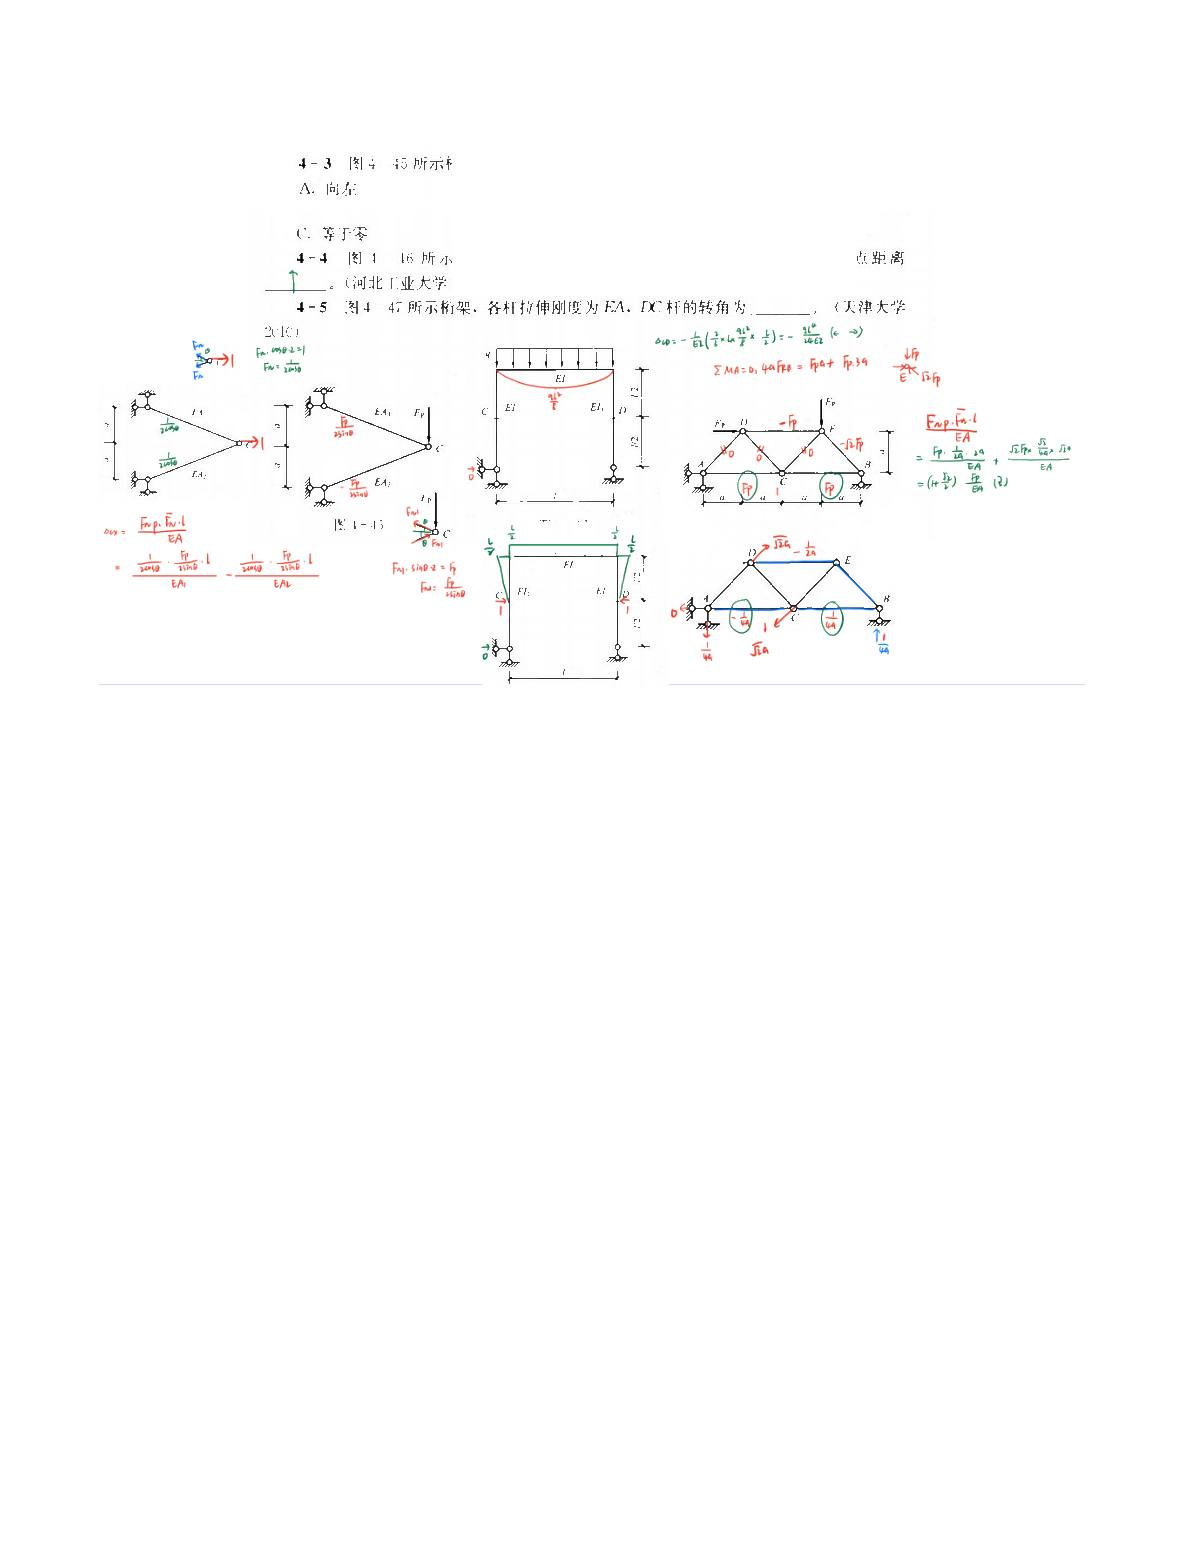
\includegraphics[width=0.92\textwidth]{figures/src29_p002.jpg}
\caption{【第9次作业笔记】 位移计算(1) 第 2 页清理图形页}
\end{figure}
\subsection*{第 3 页转写}
46

i

ii

i

嗲

i

可 

Mp

in

ijii

t

n 

477

国一点出

一点

 

m

zatm.com

品2m

i

t

Mtmyqq

MP

点in

舏

ixaxqixaxjxytifiaxiizaxiiiaxixzaxjn.iq

i

垰 

咋黙

m

t m t qa 0

48

ii

Tie

A

A

lox42 4U 40 Q10

mdij fi  140

 就 

i 钍i8   器

这

49

o

i

0

0

2to i

o i

o

i

5

t q t

t

ii

iti

2xtxl

itiqxztaxtxi.cn

2

2taD
\begin{figure}[H]\centering
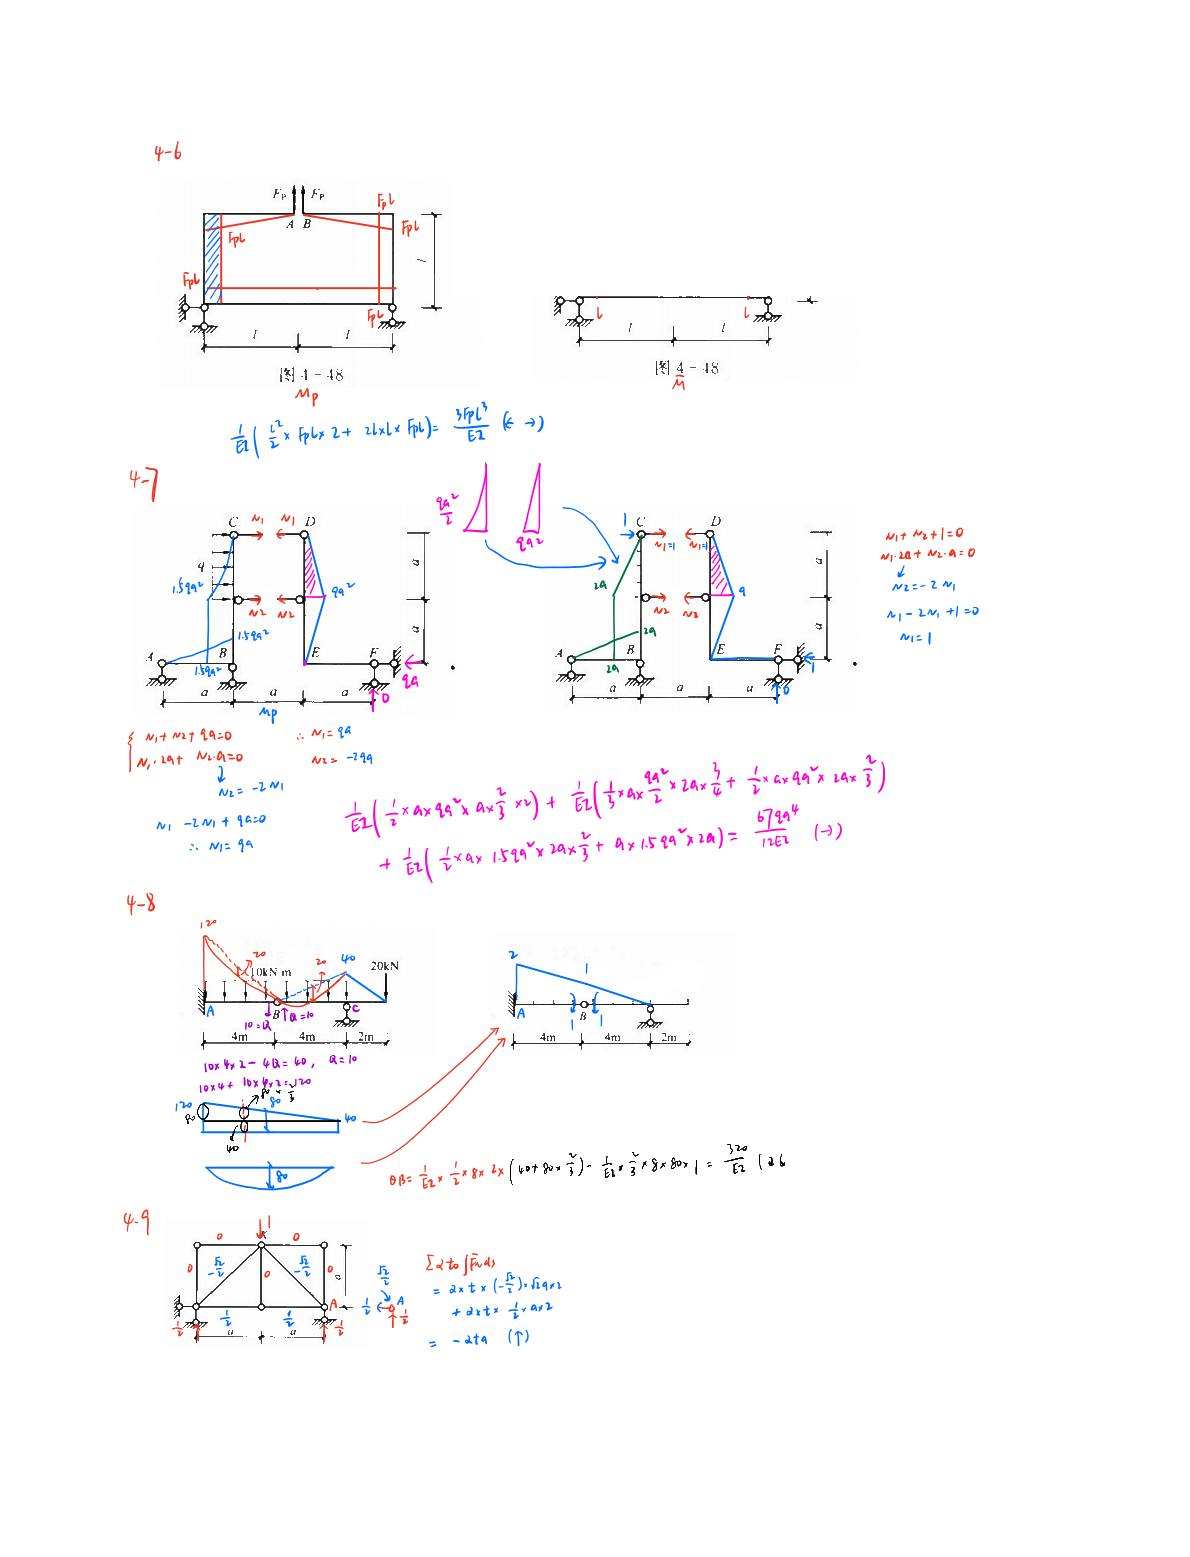
\includegraphics[width=0.92\textwidth]{figures/src29_p003.jpg}
\caption{【第9次作业笔记】 位移计算(1) 第 3 页清理图形页}
\end{figure}
\subsection*{第 4 页转写}
qa

++[nxa+ 2*a+ y+ u*g-

FP

Eup

Fmp. Cosd -2 + Fp=0

Fy-   x 2 + Fp=0

3mx4

EA

EA

LEA

3mx4
\begin{figure}[H]\centering
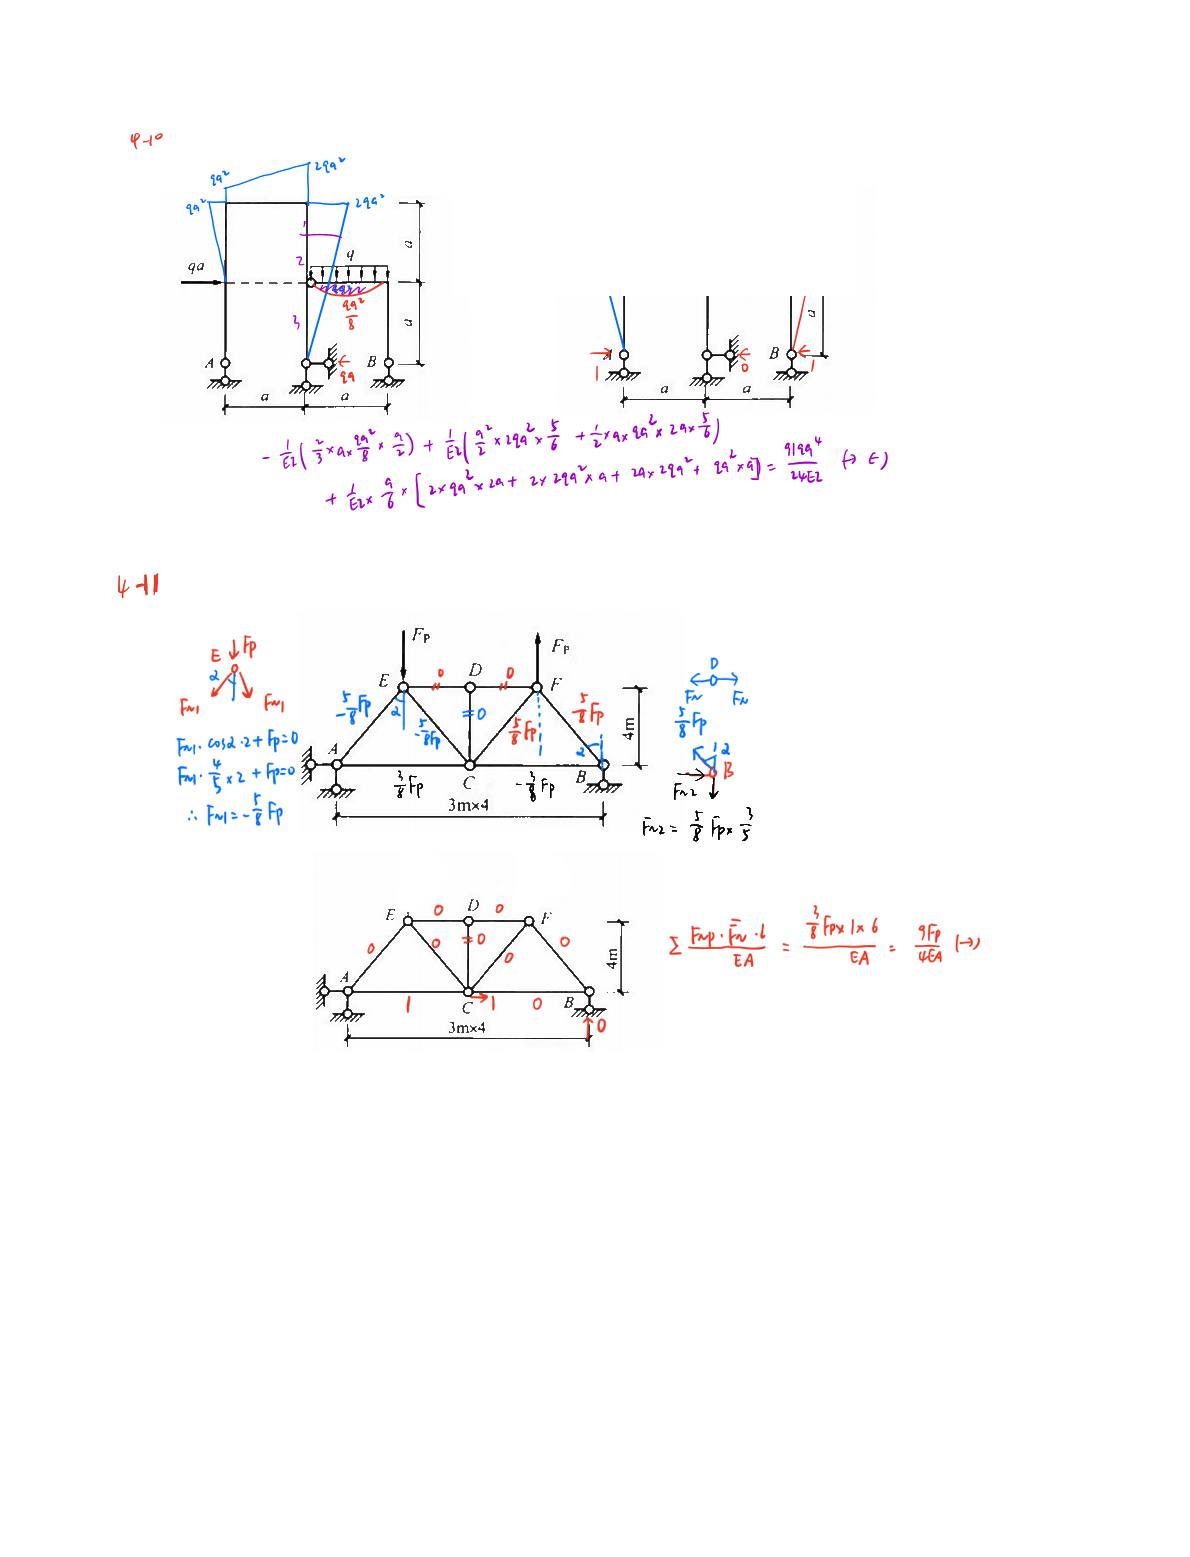
\includegraphics[width=0.92\textwidth]{figures/src29_p004.jpg}
\caption{【第9次作业笔记】 位移计算(1) 第 4 页清理图形页}
\end{figure}
\subsection*{第 5 页转写}
4-12图4-54所示结构由于支座A沉降1cm引起截面C的转角c

重)

庆大学2012）

4-13图4-55所示多跨静定梁支座A发生线位移a=10mm，转角位移=0.001rad，

图中[=10m，则铰B两侧截面的相对转角为

（中南大学2009）

1cm

4m

12m

图4-54

图4-55

Ix Dct Fe. CsD

I$\times$0B+ Fr-c=0

Ix0c+ 1m1x Ix02m=0

0= (000$\times$7 + hg01x0l *$\mu$\% + 1$\alpha$x

-- (5)

0b= - 3x103 (2 l)

4-14

计算图4-56所示结构由于支座移动产生的铰C的角位移。（湖南大学2008）

4-15求图4-57所示结构A点竖向位移$\triangle$vA，EI=常数。（西南交通大学2007)

0.01m

4m

2m

图4-56

图4-57

IxDtt FrLc0

.. 1xBc+ (-t m) 0.02m=0

. 9c= 333x 10-3 ra4

+ x+*[

34t *
\begin{figure}[H]\centering
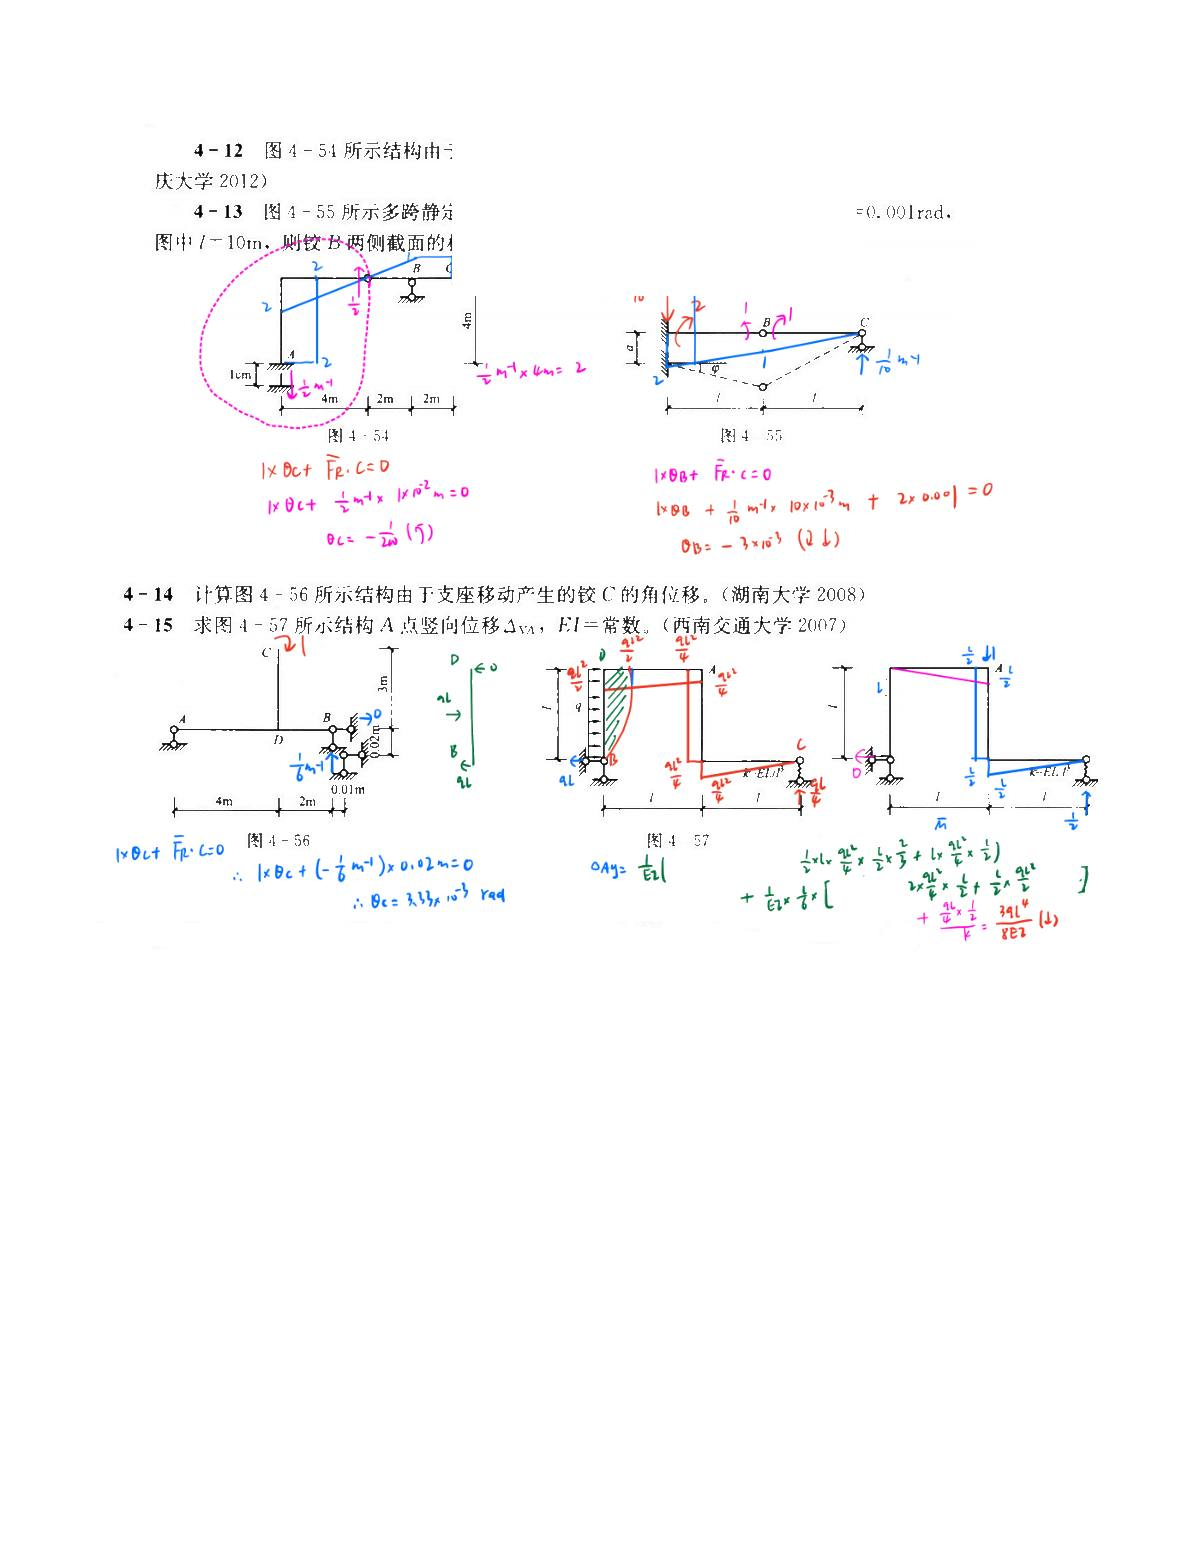
\includegraphics[width=0.92\textwidth]{figures/src29_p005.jpg}
\caption{【第9次作业笔记】 位移计算(1) 第 5 页清理图形页}
\end{figure}
